\section{Máquinas de Turing}
\subsection{Máquinas de Turing (1)}
\begin{easylist}[itemize]
& Las máquinas de Turing son un mecanismo de cómputo muy sencillo de definir. Sin embargo, son tan potentes como cualquiera de los lenguajes de programación que usamos hoy en día. Por ser de demasiado bajo nivel, no resultan prácticas para programar. Su utilidad es en el sentido contrario: gracias a ser tan simples, resulta más fácil demostrar que algo no se puede resolver con ellas. Y gracias a su equivalencia a los lenguajes de programación, facilitan demostrar que un cierto problema no se puede resolver con ningún lenguaje de programación.

& Más adelante, definiremos el concepto de lenguaje decidible como aquél reconocible por una máquina de Turing de parada segura.

& Una de las particularidades de las máquinas de Turing es que tienen un dispositivo de memoria de tamaño infinito. Eso puede parecer no razonable si queremos usarlas para representar qué cosas podemos decidir o computar y cuáles no con nuestras máquinas reales.

& Las máquinas reales tienen memoria finita. Por tanto, esencialmente, se pueden describir mediante un autómata finito determinista. Cada una de sus configuraciones estará representada por un estado, y un cambio de configuración corresponde a una transición entre estados. Aún así, hay razones que llevan a preferir no definir los lenguajes decidibles como aquellos decidibles como aquellos reconocibles por autómatas finitos deterministas. 

& En primer lugar, nótese queM en una máquina con, al menos 1 GB de memoria tendrá, al menos, $2^{23}$ bits; y, por tanto, al menos, tendrá $2^{2^{23}}$ configuraciones posibles (estados). Ese número es mucho mayor que el número de átomos en el universo (sobre $10^{77}$).

& Por tanto, no tiene sentido describir el comportamiento de nuestras máquinas como el de un mecanismo que no es transportable a la vida real. Además, si definimos \textit{lenguaje decidible} como aquel reconocible mediante un DFA, sacaremos conclusiones que no nos parecen razonables.

& Por ejemplo, concluiríamos que el lenguaje $\{a^n b^n\}$ no es decidible. Sin embargo, todo informático afirmará que sabe escribir un programa que decida si tenemos tantas $a$s como $b$s en una cadena de entrada. Por estos motivos, y porque la memoria disponible en las máquinas que usamos aumenta, se suele considerar como algoritmo a la combinación de un control de ejecución finito y memoria infinita.

& Vamos a ver más en profundidad las máquinas de Turing. Estas tienen un grafo de estados y transiciones como en los DFA. Pero, además, tienen lo que llamaremos \textit{cinta}, que es una palabra con infinitas posiciones.

& Para que el autómata maneje este dispositivo, en todo momento hay un apuntador a una de las posiciones de la cinta que llamaremos \textit{cabezal}.

& Las transiciones del autómata tendrán una condición para su ejecución que será que el símbolo guardado en la posición apuntada por el cabezal tenga que ser uno concreto.

& Además, cada transición tendrá una acción indicando qué símbolo hay que escribir en la posición apuntada por el cabezal, y si queremos mover el cabezal a derecha, izquierda o dejarlo quieto.

& Inicialmente, la máquina se encuentra en el estado incial, el cabezal apunta a la posición $1$, y en la cinta se halla la palabra de entrada de la máquina, empezando por la posición $1$.

& En la posición $0$ se halla un símbolo especial que no forma parte del alfabeto de entrada, y que llamaremos \textit{símbolo de marca de inicio} ($\vartriangleright$). Si lo gestionamos bien, siempre que veamos este símbolo, sabremos que nos encontramos lo más a la izquierda posible de la cinta.

& Después del último símbolo de la entrada, nos aparece un símbolo que llamaremos \textit{símbolo de blanco} o, simplemente, \textit{blanco} (\textblank). A partir de ese punto, todos los símbolos que aparecen son blancos.

& La máquina empezará su ejecución. Se irán ejecutando transiciones cuando se cumplan sus condiciones; como consecuencia, el cabezal se irá desplazando y, a su vez, se modificará el contenido de la cinta.

& Los símbolos que se escriban pueden ser del propio alfabeto de entrada pero también pueden no serlo. La palabra de entrada será aceptada si, finalmente, llegamos al único estado aceptador que tendrá la máquina y que marcaremos como en los DFA.

& Vamos a ver un ejemplo más concreto. Queremos construir una máquina de Turing que reconozca el lenguaje $\{w \# w \colon w \in \{0, 1\}^*\}$.

& Si la palabra efectivamente es del lenguaje, entonces la cinta tendrá este aspecto: $\vartriangleright\; 0\;1\;1 \cdots \#\; 0\;1\;1\cdots \blanco\; \blanco\cdots$, y el cabezal apuntará al primer símbolo. 

& Nos interesa ir comprobando que los símbolos de las correspondientes posiciones coinciden. Lo que haremos será recordar, mediante los estados, qué símbolo se encuentra al principio; nos moveremos hasta el principio de la segunda parte y veremos si también se halla el mismo símbolo al principio. Y, así, sucesivamente con los siguientes símbolos.

& Pero para que la máquina pueda saber qué parte de las palabras ha sido ya comprobada, iremos sustituyendo los símbolos ya tratados por símbolos nuevos a modo de marca. Por tanto, lo que haremos es: leer el primer $0$, marcarlo como $0'$ y movernos a la derecha hasta saltar el separador y recordando que hemos visto un $0$. Al ver el otro $0$, lo marcamos también y volvemos atrás saltándanos el separador hasta encontrar nuevamente la marca inicial.

& Ahora leemos un $1$, lo marcamos y vamos hacia la derecha saltándonos el separador y las marcas que encontremos, recordando que hemos visto un 1. Al comprobar que aquí hay un $1$, lo marcamos y volvemos atrás, y así, sucesivamente, hasta que hayamos comprobado que ambas palabras son iguales.

& Aquí tenemos la representación de la máquina de Turing.

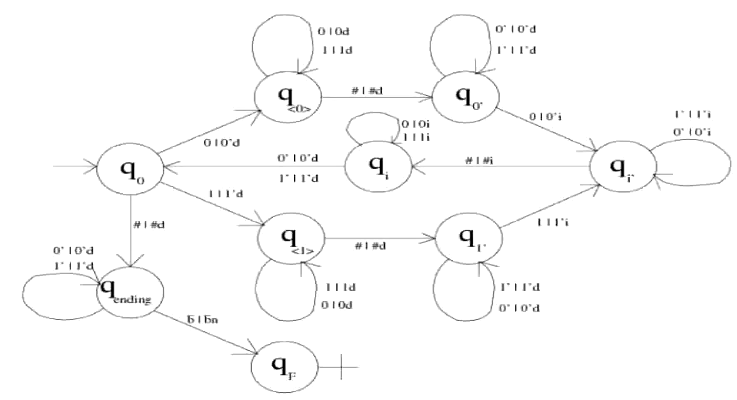
\includegraphics[width=0.8\textwidth]{t7-1.png}

& El estado inicial es $q_0$; el aceptador es $q_F$.

& Las transiciones están etiquetadas con:
&& Por un lado, el símbolo de condición para que se ejecute que es el símbolo que esperamos ver en la cinta.
&& Por otro lado, la acción que consta de qué símbolo se escribe en la cinta y si movemos el cabezal a la derecha, en este caso, o a la izquierda o no lo movemos ($d$, $i$, $n$).

& Desde el estado inicial, si leemos un $0$, lo marcamos con $0'$ y vamos hacia la derecha. Este estado $q_{<0>}$ recuerda que hemos visto un $0$, y va saltando (el bucle) símbolos hasta que lee el símbolo separador; después, va saltando símbolos marcados esperando ver, finalmente un $0$. Ese $0$ se marca y se inicia el proceso de retorno hacia la izquierda. Nos saltaremos los símbolos marcados a la derecha del separador ($q_{i'}$), luego el símbolo separador, y, después, los no marcados de la izquierda ($q_i$) hasta que encontremos, nuevamente, el símbolo marcado. En ese momento (de $q_i$ a $q_0$), nos movemos una posición a la derecha y reiniciamos el proceso.

& El caso en que veamos un $1$ desde $q_0$ se trata de forma análoga.

& Cuando vemos el separador desde $q_0$, señal de que ya hemos marcado todos los símbolos a la izquierda del separador. Para terminar de asegurarnos de que la palabra es del lenguaje; bastará con que comprobemos que todos los símbolos a la derecha del separador también han sido marcados. Esto es lo que hace $q_\text{ending}$. Cuando vemos el símbolo de blanco, saltamos a estado aceptador ($q_F$).

\end{easylist}





\subsection{Máquinas de Turing (2)}
\begin{easylist}[itemize]
& En esta sección vemos una formalización de las máquinas de Turing y definimos lenguajes decidibles, lenguajes semidecidibles y funciones computables.

& Las máquinas de Turing se pueden representar como una tupla con los siguientes elementos: $\langle Q, \Sigma, \Gamma, \delta, q_0, q_F\rangle$. Donde $Q$ es el conjunto de estados, $\Sigma$ es el alfabeto de las palabras de entrada, $\Sigma$ es el alfabeto de cinta, $\delta$ la función de transición, $q_0$ es el estado inicial y $q_F$ es el estado aceptador.

& El alfabeto de cinta siempre contiene al alfabeto de entrada y, adicionalmente, al símbolo de inicio de cinta y al símbolo de blanco. Estos dos no pertenecen al conjunto de entrada; por eso ponemos unión disjunta: $\Sigma \uplus \{\vartriangleright, \blanco \} \subseteq \Gamma$. Por supuesto, el alfabeto de cinta puede contener más de símbolos a parte de todos estos.

& La función de transición nos dice para cada estado que no sea el aceptador y cada símbolo de cinta, a qué otro estado vamos a parar, qué nuevo símbolo se escribe en la cinta y hacia dónde movemos el cabezal con opciones: \textit{izquierda}, \textit{derecha} y \textit{no mover}. Esto es: $\delta \colon Q - \{q_F\} \times \Gamma \to Q \times \Gamma \times \{i, d, n\}$.

& La función de transición es parcial: es decir, pueden no estar definida para todos los estados y símbolos posibles.

& También es posible considerar el caso no determinista. En tal caso, la función de transición ya no sería necesariamente una función, sino un subconjunto del producto cartesiano de todos los conjuntos anteriores.

& Una configuración de una máquina de Turing es un estado global en que esta se puede encontrar en algún momento. La configuración describe no sólo al estado, sino también al contenido de la cinta y a la posición del cabezal.

& El contenido de la cinta es, en realidad, infinito. Sin embargo, tan solo un número finito de sus posiciones contendrán símbolos que no sean blancos. Ya que, en un tiempo finito de ejecución, tan solo se han podido modificar un número finito de posiciones. Por ese motivo, para describir el contenido de la cinta, basta con una palabra finita.

& Usualmente, describimos una configuración del modo $w_1qw_2$. El contenido de la cinta antes del cabezal es $w_1$, el estado en que se encuentra la máquina es $q$, y $w_2$ es el contenido de la cinta desde el cabezal en adelante. En particular, el primer símbolo de $w_2$ es el apuntado por el cabezal. Se asume que más allá de $w_2$ hay blancos. Por ese motivo, esta configuración se considera equivalente a $w_1 q w_2 \blanco \blanco \blanco$ (todos los blancos que queramos).

& La función de transición $\delta$ también se puede representar mediante un sistema de reescritura con reglas que se aplican sobre configuraciones.

& Nótese que una transición de desplazamiento hacia la derecha se puede representar mediante la regla $qa \to bq'$. La regla se aplica sobre una configuración si el estado es $q$ y el símbolo apuntado por el cabezal es $a$. Reemplaza localmente el símbolo $a$ por $b$ y mueve el cabezal hacia la derecha, y cambia el estado a $q'$.

& De manera similar, si la transición no desplaza el cabezal, esta regla nos permite representarla: $qa \to q'b$.

& En el caso de transiciones que desplazan el cabezal hacia la izquierda, la situación se complica ligeramente, porque la regla necesita saber qué símbolos se encuentran a la izquierda del cabezal. Por ese motivo, transiciones de este estilo se representan mediante tantas reglas como símbolos tiene el alfabeto de cinta. En esta descripción, estamos asumiendo que $a_1$ hasta $a_n$ son los símbolos del alfabeto de cinta: $a_1 q a \to q' a_1 b, \dots, a_n q a \to q' a_n b$.

& Definimos el lenguaje aceptado o reconocido por una máquina de Turing como el conjunto de palabras que nos llevan a estado aceptador. Esto es: $\mathcal L(M) = \{w \in \Sigma^* \colon \exists w_1, w_2 \in \Gamma^*, n \in \mathbb N \colon \vartriangleright w  \blanco^n \to_\delta ^* w_1 q_F w_2\}$. Más concretamente, son aquellas palabras sobre el alfabeto de entrada tales que, añadiendo el símbolo de inicio de cinta a su izquierda y un número suficiente de blancos a su derecha pueden acceder por reescritura de la función de transición hasta una configuración cuya estado sea aceptador ($w_1 q_F w_2$).

& Definimos la función computada por una máquina de Turing del siguiente modo. Un elemento $x$ tiene como imagen $y$ si, teniendo $x$ como entrada, la máquina llega a estado aceptador dejando $y$ en la cinta. Más concretamente, si $x$ e $y$ se forman sobre el alfabeto de entrada y, además, tras añadir el símbolo de inicio de cinta a la izquierda de $x$ y suficientes blancos a su derecha accedemos a una configuración con estado aceptador y que contenga $y$ entre el primer y segundo símbolo fuera del alfabeto de entrada ($\alpha_1 y \alpha_2 w')$, entonces decimos que $y$ es la imagen de $x$ por la función computable por la máquina.

& Fijaos que, mediante la aplicación de la regla adicional $q_F \to \Gamma$, estamos borrando el estado aceptador de la configuración para poder hablar únicamente del contenido de la cinta. Es decir: $\varphi_M (x) = y$ es equivalente a $x,y\in\Sigma^*$ y, además, existen $\alpha_1, \alpha_2 \in (\Gamma - \Sigma), w' \in \Gamma^*, n \in \mathbb N$ tales que $\vartriangleright x  \blanco^n \to_{\delta \cup \{q_F \to \lambda \}} \alpha_1 y \alpha_2w'$.

& No es difícil convencerse de que el dominio de la función computada por la máquina $M$ es justamente el lenguaje reconocido por $M$: $\textrm{Dom}(\varphi_M) = \mathcal L (M)$.

& De este modo, denotamos que la imagen de $x$ por $\varphi_M$ está definida. Es decir, que existe una $y$ que es su imagen: $\varphi_M (x) \downarrow \equiv \exists y \colon \varphi_M (x) = y \equiv x \in \mathcal L (M)$.

& Decimos que una configuración es terminal si no se le puede aplicar ninguna regla: $\nexists w' \in \Gamma^* \colon w  \blanco \to _\delta w'$.

& De este modo, denotamos que la máquina $M$ con entrada $x$ termina su ejecución en algún momento: $M(x) \downarrow$. Es decir, que existe $n \in \mathbb N$ y una configuración terminal $w$ tal que $\vartriangleright x  \blanco^n  \to _\delta ^* w$.

& Nótese que toda configuración aceptadora es terminal por tanto, si la imagen de $x$ está definida, entonces la máquina para con entrada $x$: $\varphi_M (X) \downarrow \implies M(x) \downarrow$. Sin embargo, la implicación contraria no es necesariamente cierta, ya que puede haber configuraciones terminales que no sean aceptadoras. Símplemente puede ocurrir que no se pueda aplicar ninguna regla por no haber más transiciones definidas.

& En el caso en que $\varphi_M(x)$ esté definida, entonces, por $M(x)$ también denotamos $\varphi(x)$.

& Definimos un lenguaje como decidible si existe una máquina de Turing que lo reconoce y que para con toda entrada. En tal caso, decimos que la máquina decide el lenguaje. Esto es, $L$ es decidible ($L \in \textrm{Dec}$) si existe una máquina de Turing $M$ tal que $\mathcal L(M) = L$ y $M$ para con toda entrada.

& Definimos un lenguaje como semidecidible o recursivamente numerable si existe una máquina de Turing que lo reconoce. En tal caso, decimos que la máquina semidecide el lenguaje. Así pues, semidecidir y reconocer son palabras sinónimas. Esta máquina puede no parar con aquellas entradas que no sean del lenguaje. En definitiva: $L$ es semidecidible ($L \in \textrm{semi-Dec}$) si $\exists M \in \textrm{TM}$ tal que $\mathcal L(M) = L$.

& Definimos una función como computable si existe una máquina que la computa. En tal caso, decimos que esa máquina es una implementación de la función o que computa la función: $f\colon \Sigma^* \to \Sigma^*$ es computable si y solo si existe una máquina de Turing $M$ tal que $\varphi_M = f$. Nótese que $f$ no necesariamente debe ser total, y que otra definición alternativa a computabilidad es: $f$ es computable si y solo si para toda entrada del dominio $w$, $M(w) \downarrow$ en $q_F$ de manera que $M(w) = f(w)$. Cabe notar que, para las entradas $w$ que no son del dominio, puede pasar que $M(w) \uparrow$ o bien $M(w) \downarrow$ en estado $q_F$. Solo nos importan las palabras del dominio


\end{easylist}
